\documentclass[11pt]{article}
\pdfinfoomitdate=1
\pdftrailerid{}
\usepackage[T1]{fontenc}
\usepackage[utf8]{inputenc}
\usepackage{lmodern,microtype,amsmath,amssymb,amsthm,booktabs,tabularx,enumitem}
\usepackage[margin=1in]{geometry}
\usepackage{xcolor,tikz}
\usetikzlibrary{arrows.meta,positioning}
\definecolor{ink}{HTML}{172C42}
\usepackage[colorlinks=true,linkcolor=ink,citecolor=ink,urlcolor=ink]{hyperref}
\usepackage{url}
\usepackage[numbers,sort&compress]{natbib}
\usepackage{titlesec}
\titleformat{\section}{\large\bfseries\color{ink}}{\thesection}{0.7em}{}
\titleformat{\subsection}{\normalsize\bfseries}{\thesubsection}{0.6em}{}
\setlist{nosep,leftmargin=*}
\setlength{\parskip}{0.35em}
\setlength{\parindent}{0pt}
\setlength{\emergencystretch}{2em}
\newtheorem{proposition}{Proposition}
% Generated from retained evidence; regenerate with tools/check.py --refresh.
\newcommand{\ModelStates}{5,508}
\newcommand{\ModelTransitions}{132,192}
\newcommand{\TraceCount}{118}
\newcommand{\MatchedSteps}{312}
\newcommand{\ContractTests}{143}
\newcommand{\ProofCount}{7}
\newcommand{\UpstreamTests}{76}
\newcommand{\PairedTests}{20}
\newcommand{\IntegrationSummary}{The integrated evidence snapshot passes 95 native tests, including all six opt-in chain tests, and 20 selected process scenarios covering authenticated transport, bilateral isolation, earned-child recovery, refund resolution and custody. The final source differs only by removal of a redundant dereference, checked by strict Clippy, four affected unit tests and a fresh authenticated payout/refund run. All roles remain under author control. Broader formal-source mapping, file-hygiene, hosted and deployment qualification remain open.}

\hypersetup{pdftitle={Chio: A Peer-to-Peer Economy of Verifiable Work},pdfauthor={The Chio Project}}
\title{\vspace{-2em}\textbf{Chio: A Peer-to-Peer Economy\\of Verifiable Work}}
\author{The Chio Project\\\small\url{https://github.com/bb-connor/arc}}
\date{October 2026}
\begin{document}
\maketitle
\begin{abstract}
An agentic web needs programs that recruit collaborators and grow across
administrative boundaries while each owner retains control over its resources.
We present Chio, a kernel interface for composing work through local
authorization and durable commitments. Its organizing rule is that plans may
evolve while issued commitments retain their authority bounds and execution
identity. Delegated work contracts subdivide an owner's allocation, select
signed offers and seal the exact receiver, input and invocation into portable
evidence. For running swarms, signed graphs grow by retaining earlier tasks,
allocations and continuation identities. Each receiver applies its own
capabilities and treaty conditions before dispatch. Under protected allocation
and receiver custody, the composition conserves declared capacity across graph
versions and prevents graph growth from refreshing a consumed invocation.
A local Rust experiment connects recursive delegation, live graph evolution
and bilateral native admission to funded work in one execution. A first result
triggers allocation of a new collaborator; after that collaborator earns its
claim, the intermediary is killed before completing its own work. The original
child claim is collected without another parent authorization, while earlier
execution evidence and continuation custody survive graph growth and restart.
This supplies an execution contract for the agentic web: programs may change
their plans while resource owners retain authority and accepted work retains
its claim.
\end{abstract}
\section{Introduction}
\label{sec:introduction}
An agent that delegates work across organizations commits resources before it
knows how the work will unfold. It may reserve funds or authorize a tool call,
then discover a task requiring another provider. Each provider must be able to
determine which actions were authorized, which ran and which earned payment
as the plan changes.

Consider a buyer who funds an API survey and a follow-on review by an
intermediary agent. After the survey identifies a problem, the intermediary
hires a specialist from its own funds. The specialist completes its task and
earns payment, but the intermediary crashes before returning a result to the
buyer. Three facts must
survive the crash: the specialist's call has already run, its payment is owed,
and the buyer's task may still be incomplete. A replacement process must recover
those facts before deciding what to do next.

Plan changes introduce a related problem. A newly signed plan may contain both
the completed survey and the new specialist task. If the signature gives every
task a fresh execution right, the survey can run twice. If the new plan replaces
the evidence for the old one, a receiver may lose the terms under which the
survey ran. Valid signatures on each version do not, by themselves, establish
continuity between them.

We present Chio, a protocol and runtime kernel that preserves this continuity.
Its unit of composition is a \emph{work commitment}: signed records that bind
one selected invocation to a bounded allowance, the receiving owner's
authorization and, for paid work, its settlement terms. The records refer to
the same invocation by authenticated identifiers and digests. Each authority
checks the references relevant to its decision and retains the state needed
to prevent that decision from being spent twice.

The construction separates the identity of a task from the version of the plan
that contains it. An extension retains earlier tasks and allocations. A receiver
records the use of each execution right under a stable identity, so a signature
on a later plan cannot make that right unused again. Settlement reserves funds
for each agreement separately; once acceptance is recorded, a parent failure
cannot release a child's earned reserve. These rules permit incremental work
without a transaction that locks every participant at once.

Each receiving kernel admits work under its owner's capabilities, policies and
treaties. Foreign agreements supply evidence checked under locally selected
authority. We call this arrangement \emph{programmable sovereignty}: owners
express conditions for cooperation in verifiable agreements and enforce them
at their own resources.

We specify the records and transitions, establish a preservation result under
explicit trust assumptions, and implement the construction in Rust. Evaluation
follows the API example through graph growth and process loss, tests adversarial
substitutions, and compares the financial rules with transactional escrow and
ERC-8183.

\section{Resources, authority and trust}
\label{sec:sovereignty}
An \emph{agent} proposes work. A \emph{resource owner} decides which work may use
its tools, data or funds. A provider executes a task through a \emph{receiving
kernel}, which validates capabilities, runs policy and guard checks, and records
its decisions. The kernel is trusted for these operations. Host isolation and
tool confinement must make it the effective mediator of the protected resource.

An owner can authorize an agent to use part of a resource allocation. That agent
is the allocation's \emph{holder}; it may subdivide the allowance or select a
provider within its terms. The owner's \emph{allocator} records these choices.
A paid task also names a payer, a verifier that judges the result, and an escrow
that reserves and transfers funds. One organization may perform several roles.
Couriers need not be trusted: the receiver checks signatures under local
configuration.

\subsection{Admission under local authority}
A work agreement describes what the parties intend to exchange. Admission is
the receiver's decision to allow a particular invocation. The receiver loads
trusted issuers, capabilities, policy, treaties and replay state from stores
controlled by its owner. A request can refer to these authorities but cannot
install them.

A bilateral treaty records the conditions under which two participants
cooperate. The receiver checks the configured participants' signatures over the
same statement, the permitted action and validity period, and the invocation
and continuation records required by the treaty. A continuation identifies a
right to perform work under that agreement. Its use is recorded so that replay
cannot create another invocation. Treaty checks apply together with the
receiver's ordinary capability, revocation and guard checks.

Local authority also determines how changes take effect. Current policy can
deny a fresh call. An already admitted call has an execution history that
recovery must consult. An earned escrow claim follows the terms under which
its reserve was funded. Control over admission therefore coexists with
obligations that remain binding after admission.

\subsection{The authorities that must agree}
The protocol links three kinds of state. The allocator records which allowances
have been assigned; the receiver records which calls were admitted and what
their execution established; the escrow records which funds are reserved, earned,
paid or refunded. Each record answers a different question. In particular, an
allowance establishes a spending limit, while a deposit supplies the funds.
A refund records a financial outcome without establishing whether a tool
executed.

A \emph{protected} store is durable state controlled by the authority responsible
for that resource. All uses of the resource must consult that state. Each
delegation root has one protected allocator. Each declared pool for a work graph
has one protected sequence of graph versions, whose updates are serialized.
Each receiving key has one protected execution and budget domain. The settlement
system serializes financial transitions and couples them to actual transfers.
Copying a key and database into independently spendable forks, or provisioning
two graph sequences against the same declared pool, violates these premises.

\subsection{Failure model and meaning of verification}
Agents and couriers may be malicious. Messages may be duplicated, reordered,
delayed or lost; a process may crash between durable steps. Safety assumes
unforgeable signatures, collision-resistant canonical digests, valid clock
checks and honest enforcement by the selected resource authorities. Tools must
be confined sufficiently for their declared actions and permitted readers to
describe their effects and disclosures.

For paid work, the parties trust the agreed verifier and the rule used to
recognize a recorded settlement. \emph{Verifiable work} means work whose agreed
acceptance condition and execution evidence can be checked. A kernel receipt
authenticates the kernel's account of its mediated call; a verifier's decision
attests satisfaction of the chosen acceptance condition. Useful work depends
on choosing that condition well.

The implementation recruits from previously enrolled principals. Discovering
a task permits a new selection within the authorized set; it does not add a
trusted issuer or authorize a new reader. Appendix~\ref{app:profiles} maps these
rules to the delegation, graph-evolution and funded-work profiles used in the
experiments.

\section{The work contract}
For exposition, write an agreement as
\[
 A=(B,P,I,C,D,F,T,L),\qquad a=H(\operatorname{canon}(A)).
\]
$I$ commits the input, $C$ identifies the checker and acceptance policy, $D$
defines permitted disclosure, $F$ identifies the funding domain and terms, $T$
sets the deadlines, and $L$ names any parent agreement. Both parties sign the
same canonical agreement. This tuple is a description of the common contract,
not a replacement wire encoding. The artifact companion maps it to the
versioned implementation objects.

An agreement has three bindings. \emph{Authority binding} connects it to the
receiver's own admitted operation and bounded local grant. \emph{Result binding}
connects the exact input, output and acceptance procedure. \emph{Funding binding}
connects the agreement and result commitment to one allocation, beneficiary,
asset and amount in one settlement domain. These bindings prevent a valid
statement about one relationship from being reused as a statement about another.
They do not establish useful work independently of the acceptance procedure.

\subsection{Funding is an allocation}
The payer deposits $q>0$ units into an allocation $f$. The reference contract
derives its allocation identifier from the chain, contract address and complete
terms. The agreement digest, payer, beneficiary, verifier, asset, amount and
four deadlines are immutable. A new payer agreement cannot be funded twice
under the same payer and digest. The receiver checks the selected contract code
and observation source before relying on an allocation.

A provider does not start merely because a payer supplies a signed balance. It
requires an acceptable observation of the actual reserved allocation and a
local admission decision bound to it. The binding does not atomically fuse a
remote blockchain with a local database. Fresh observation, the deadline
margin, retained operation identity and conservative recovery are necessary.
If the chain reorganizes after an observation, the profile's finality assumption
has failed or the observation was premature. A local receipt cannot repair that.

\subsection{Acceptance is an explicit decision}
A submission commits the result and its evidence. A verifier checks the exact
agreement, allocation, input, output, checker and custody record before issuing
a decision. Missing evidence produces no decision. An available result that
fails the predicate produces rejection. These outcomes must remain distinct:
a verifier outage is not proof that the provider delivered bad work.

Off-chain artifacts use canonical JSON and Ed25519 signatures~\cite{jcs}.
The reference escrow accepts a separate EIP-712 decision~\cite{eip712}, binding
the allocation, agreement, submission commitment, decision digest, acceptance
bit, beneficiary, asset and amount. Its domain includes chain ID and contract
address. The contract verifies the pinned signer's decision, not the
application predicate. The publication artifact specifies which digests cover
bodies and which cover complete signed envelopes; those encodings cannot be
interchanged.

\subsection{A child is a separate obligation}
A parent link records provenance. It is not collateral and grants no authority.
Before hiring a specialist, the intermediary must commit funds it already
controls to a different allocation. In the opening example, the buyer deposits
100 and the intermediary deposits 60. The buyer's reserved 100 is not available
for the intermediary to pledge again. If the intermediary cannot finance the
60, this profile cannot admit the subcontract. Credit or conditional netting
would require a different contract and a different failure argument.

\begin{figure}[t]
\centering
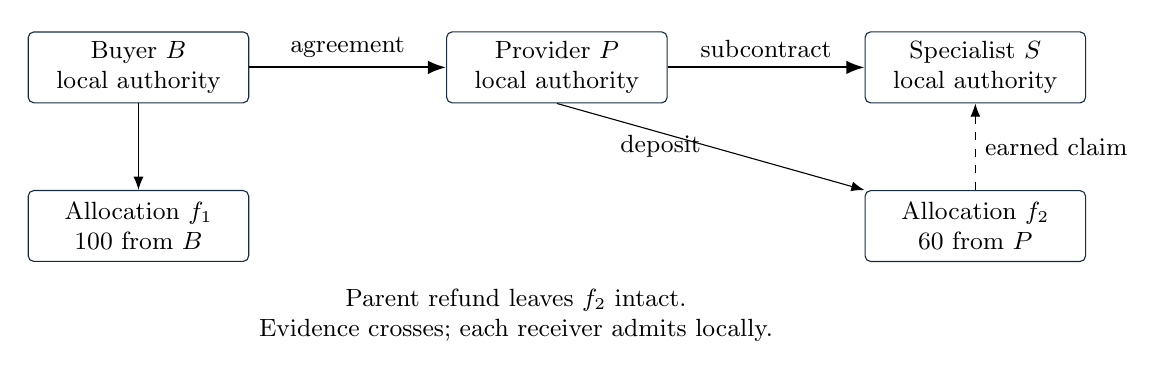
\begin{tikzpicture}[font=\small,box/.style={draw=ink,rounded corners=2pt,align=center,minimum width=2.8cm,minimum height=0.9cm},>=Latex]
\node[box] (b) {Buyer $B$\\local authority};
\node[box,right=2.5cm of b] (p) {Provider $P$\\local authority};
\node[box,right=2.5cm of p] (s) {Specialist $S$\\local authority};
\draw[->,thick] (b) -- node[above]{agreement} (p);
\draw[->,thick] (p) -- node[above]{subcontract} (s);
\node[box,below=1.1cm of b] (f1) {Allocation $f_1$\\100 from $B$};
\node[box,below=1.1cm of s] (f2) {Allocation $f_2$\\60 from $P$};
\draw[->] (b) -- (f1);
\draw[->] (p.south) -- node[left]{deposit} (f2.north west);
\draw[->,dashed] (f2) -- node[right]{earned claim} (s);
\node[align=center,below=0.22cm of f1.south east,anchor=north west] {Parent refund leaves $f_2$ intact.\\Evidence crosses; each receiver admits locally.};
\end{tikzpicture}
\caption{Work dependencies and funding dependencies differ. Each obligation has
its own backing; the figure depicts neither a shared application operator nor
an absence of shared settlement and verification dependencies.}
\label{fig:work}
\end{figure}

\section{Execution, recovery and payment}
\subsection{The native delegation boundary}
D1's receiver consumes a slot ID, payload and signed dispatch permit. The
installed guard requires a locally accepted allocator and checks the allocator,
holder and receiver signatures. It compares the exact receiver key, capability
subject, server/tool, input digest, request ID and capability digest with the
sealed selection. The capability must be issued by this receiving kernel and
contain one exact invoke grant, one invocation, and per-call and total monetary
ceilings no larger than the offer. The offer and slot must be live. Ordinary
native capability validation, revocation and policy checks still apply.

The installation API requires durable native admission and enables original
request retention. The receiver selects either the original argument envelope
or a governed-context layout; the caller cannot select a weaker interpretation.
In the composed layout the permit commits to every original tool argument,
including existing financial terms, without rewriting the tool payload. The guard revalidates before dispatch and checks the exact
JSON value after output transformations. A signed offer in D1 agrees to
accepted-output pricing: a qualifying predicate rejection withholds output and
uses the native reversible-hold path to produce a zero-charge denial. The
executed invocation remains consumed. This rule depends on the qualified
payment profile; a portable permit does not implement settlement by itself.

Sealing uses two durable steps: first freeze the exact selection, then persist
the signed permit before returning it. A crash between them can strand
capacity. Retrying returns the original stored permit once available, and
cannot replace its provider or request. Native custody, rather than a permit
cache, determines whether that request has already executed. Timeouts do not
authorize a replacement. Independent siblings can proceed from their own
allocations while the original operation is unresolved.

In the native fault experiment, the receiver process is killed after
\texttt{ToolReturnRecorded}. A second receiver cannot replace the original
allocation, but completes an already allocated sibling. Reopening the first
receiver recovers its recorded output without a fresh tool call. This cut has
recoverable evidence; it does not establish recovery from every possible cut.
An effect lacking authoritative completion evidence remains unknown. Ordinary
external effects acquire no exactly-once guarantee from the permit.

\subsection{Extending a running swarm}
S1 adds one operation to the existing swarm lifecycle. Given the expected
digest of the installed bundle and a signed candidate, the runtime store
checks both bundles with the ordinary live-authority verifier at store-owned
time. It then checks retention: the original graph envelope, nodes, edges,
joins, routes, witness chains, allocations and revocation epoch remain intact.
The candidate must add nodes within the original depth, fan-out and pool limits.
Each task has at most one allocation and continuation. Existing continuations
retain every field except the new graph digest and its signature. A new task
receives a new continuation; an old task cannot receive a new attempt identity.

In one immediate SQLite transaction, the installer compares the expected head,
archives the exact parent bundle and installs the successor. Competing proposals
against one parent cannot both commit. The archive binds the graph index to the
signed graph digest and full bundle digest. Admission uses the graph digest
already carried by the request, so an unfinished operation can still present
its original evidence after growth. Every fresh invocation also passes the
ordinary current capability, revocation and treaty gates.

The native kernel owns the single-use continuation resource by its stable ID.
A changed graph digest therefore cannot turn a consumed continuation into fresh
authority. Replaying a completed request resolves its original operation and
receipt. Revalidating an original physical claim reads its original graph and
treaty evidence. The installer does not need a joint transaction with every
running operation: additive growth leaves their allocations and identities
intact. Non-additive retirement would require a different authority boundary.

\subsection{One admission across three resource owners}
The composed adapter resides in the experimental funded receiver. Its protected
policy pins the allocator, swarm witness, treaty peer and runtime profile.
Opening the receiver installs the same delegation guard and runtime admission
hook before recovery. Removing that configuration changes the pinned policy;
losing its runtime database cannot silently provision empty custody.

The D1 slot ID equals the native request ID and S1 task ID. The S1 allocation ID
is the D1 allocation digest; both agree on amount and currency. The sealed
permit and native swarm witness bind the same capability. The signed route must
target this receiver. The existing F1 agreement signs the entire final request,
including the governed D1, swarm and treaty references. Its escrow allocation ID
therefore commits transitively to those references. These are different hash
domains joined by checked bindings, not interchangeable identifiers. The
agreement is downstream of the request, so no circular hash is required.

Before dispatch, the receiver checks treaty and capability authority separately
from observed escrow backing. One existing native operation acquires both the
treaty and swarm continuation resources. Its payment adapter compares the
governed payment context with the original retained intent, then binds the
original funding allocation to the operation and budget hold. A new graph
member receives neither a capability nor funds merely by appearing in a graph.

A receiver-local pre-settlement statement authenticates the retained execution
and output before a funded decision. For a federated invocation, export
revalidates the original frozen treaty, participants and admission time against
the content-addressed native outcome. It does not ask for a new remote
co-signature, imply delivery to the remote party, or settle payment. The agreed
checker and escrow decision establish the earned claim. Final bilateral
receipt delivery remains a separate operation.

The commit order is seal, bind the funded agreement, deposit backing, install
checked growth, admit and dispatch, then record acceptance. No distributed
transaction spans those owners. A crash between steps may strand unused
capacity or funds until the existing refund rules apply. It cannot silently
replace the original receiver, request or allocation.

\subsection{The funded state machine}
F1's financial state machine has seven states after funding:
\[
\textsf{Funded}\to\textsf{Submitted}\to
\begin{cases}
\textsf{Payable}\to\textsf{Paid},\\
\textsf{Rejected}\to\textsf{Refunded}.
\end{cases}
\]
A funded or submitted job without a decision can become
$\textsf{TimedOut}$ and then $\textsf{Refunded}$. There is no edge from
$\textsf{Payable}$ to timeout or refund.

Let $t_s<t_c<t_r<t_f$ denote submission, challenge, resolution and refund
boundaries. The beneficiary submits by $t_s$. A first verifier decision is
recorded only when $t_c<t\leq t_r$. Without a decision, refund is allowed only
when $t>t_f$. The interval before decision is a timing boundary, not a claim
that F1 implements a public challenge court. The exact verifier decision may
be carried by any courier. Its first valid recording determines acceptance;
an identical replay changes nothing, and a conflicting replay fails.

A claim is \emph{earned} here when an accepting decision has been recorded in
the settlement state under the selected finality rule. Merely producing an
output or obtaining an off-chain signature does not earn this right. After
that transition, the beneficiary may withdraw without a new payer signature.
The reference contract imposes no later expiry on an earned withdrawal.
Administrative pause and verifier-registry changes govern new funding and do
not revise an existing claim. The recipient still needs transaction inclusion,
fees and a functioning asset contract.

Local execution proceeds under its own durable operation identity. The kernel
commits admission before dispatch, retains observed output and produces signed
evidence. The funded integration carries the original allocation, operation,
hold and authorization identifiers through verification and recovery. Recovery
reopens that history; it must not mint a fresh admission simply because a
response was lost. A return whose occurrence cannot be established remains an
unknown terminal. A later financial resolution has its own authority and does
not rewrite the original observation.

For actual rail transactions, the research implementation records the exact
signed transaction before broadcast. After a crash it reobserves or rebroadcasts
those same bytes. A changed nonce, transaction or funding context is not an
ordinary retry. This approach handles particular durable cutpoints; it is not
an exactly-once guarantee for arbitrary tool effects.

\subsection{Successful exchange and failed intermediary}
In a successful exchange, the buyer and provider sign the terms, the buyer
funds $f_1$, and the provider admits one bound operation. The result and custody
record identify the exact submitted bytes. The verifier reruns the selected
check, records acceptance, and the provider withdraws 100. An offline reader
can verify the signed evidence without possessing either party's private keys;
current spendability still requires settlement state.

For the failed intermediary, the specialist's 60-unit child claim becomes
$\textsf{Payable}$ but remains uncollected. The parent produces no eligible
submission and its 100 returns to the buyer after timeout. The specialist then
withdraws the original 60. The provider bears the loss because it funded the
child. This is neither a transfer of the buyer's risk to an unpaid specialist
nor a claim that failed computation is free.

If instead the verifier never records a child decision, the child may time out
and refund its payer despite the specialist having performed work. F1 protects
recorded earned claims; it cannot guarantee timely adjudication against its own
failed verifier. That distinction is the decisive difference between financial
safety and an unconditional promise to pay for every useful result.

\section{The preservation property}
\label{sec:preservation}
The protocol has a single composition criterion: every allowed change must
preserve the bounds and identity of existing commitments. Three invariants
make this criterion precise.

\subsection{Capacity is allocated once}
Let $B_D$ be a delegation root's ceiling, $b_v$ the ceiling of a leaf and $U_v$
the unused remainder of an internal slot. Subdivision preserves
\begin{equation}
 \sum_{\mathrm{leaves}\ v}b_v+\sum_{\mathrm{internal}\ v}U_v=B_D,
 \qquad b_v,U_v\geq0. \label{eq:delegation}
\end{equation}
It moves capacity from a parent remainder into a child, without changing the
sum. Internal slots cannot execute; selection and sealing change no ceiling.
Declared effect and reader inclusion, decreasing expiry and decreasing depth
extend transitively along the allocation tree. With the bound one-invocation
capabilities and native charge enforcement, admitted leaf charges fit those
ceilings.

For a swarm lineage, let $A_i$ be the set of uniquely identified allocations
in $G_i$, with fixed ceiling $b(a)$ and original declared pool $B_G$.
Every checked extension satisfies
\begin{equation}
 A_i\subseteq A_{i+1},\quad
 b_{i+1}(a)=b_i(a)\ (a\in A_i),\quad
 \sum_{a\in A_{i+1}}b(a)\leq B_G. \label{eq:growth}
\end{equation}
A single protected lineage per declared pool, with a serialized head,
establishes the domain of this bound. Because earlier allocations are
retained, $\bigcup_{i=0}^n A_i=A_n$: the latest bound also covers every allocation
ever installed. These are capacity bounds; deposited assets have a separate
accounting invariant.

\subsection{Funds follow their own allocation}
For each accounted endowment $u$, fix deposited funds $D_u$ with no further
deposits into that accounting cohort. Let $A_u$ be its available balance,
$L_u$ its locked funds, and $P_u,R_u$ its paid and refunded outflows. Then
\begin{equation}
 D_u=A_u+L_u+P_u+R_u,\qquad A_u,L_u,P_u,R_u\geq0.
 \label{eq:conservation}
\end{equation}
Reservation moves funds from $A_u$ to $L_u$; payment or refund moves an
allocation's locked funds once to the corresponding outflow. Each transition
preserves the sum and nonnegativity. Returned cash remains an outflow in this
cohort. A later deposit is accounted as another endowment; it neither resets
these accounts nor releases their still-locked allocations.

An earned allocation remains in $\{\textsf{Payable},\textsf{Paid}\}$.
A transition on another allocation leaves it unchanged. Thus a parent refund
cannot consume an earned child's reserve. Eventual withdrawal also requires
the beneficiary's key, available evidence, transaction inclusion and a
functioning asset.

\subsection{Compose through the original invocation}
\begin{proposition}[Preservation under evolving work]
Assume the protected allocation, graph, receiver-custody and settlement domains
of Section~\ref{sec:sovereignty}, the authenticated bindings of
Section~\ref{sec:contract}, and the transitions of Section~\ref{sec:execution}.
Begin with validly provisioned roots, verified initial graphs and funded
accounts. Within those declared domains, every finite interleaving of valid
subdivision, sealing, graph growth, native execution, recovery and settlement
preserves the following properties:
\begin{enumerate}
 \item Declared delegation and swarm capacity remain within their original
       bounds; paid plus refunded funds never exceed deposited backing.
 \item A sealed invocation retains its selected receiver, capability, input,
       effect and request. Graph growth and replay grant it no additional
       native invocation right.
 \item A recorded earned child claim retains its original terms and remains
       payable or paid through any parent failure, completion or refund.
\end{enumerate}
\end{proposition}

\begin{proof}
Initially, a new root has all its capacity in one leaf, a verified graph fits
its declared pool, and a fresh funded endowment has
$(A_u,L_u,P_u,R_u)=(D_u,0,0,0)$. No execution right has been consumed or payment
earned. The properties hold in this initialized state.

Induct over the interleaving. A subdivision changes only the parent's remainder
and its new child, preserving (\ref{eq:delegation}). A selection changes no
capacity. Sealing freezes the selected binding before evidence escapes.

A graph extension preserves every earlier allocation and checks
(\ref{eq:growth}) before committing its new head. The old continuation keeps its
resource identity. Exact historical lookup preserves the artifacts used by
an old request; a new graph signature cannot cause native custody to acquire
that resource as a second invocation.

Admission compares the request with the sealed permit, native capability,
graph task, route and treaty. The funded agreement authenticates that same
request. A substituted object either fails the binding or requires a different
authorized commitment. Native recovery resolves the original operation, hold
and continuation claim. Refusal, expiry and revocation can prevent fresh work;
they do not create a replacement invocation from the old commitment.

Financial transitions preserve (\ref{eq:conservation}). Their allocation
identity confines each transition to its own reserved funds. A parent
transition cannot change the child; a child transition after acceptance stays
inside $\{\textsf{Payable},\textsf{Paid}\}$.

These cases cover the allowed transitions. They remain valid when interleaved
because additive growth retains the resources on which old execution depends,
and each scarce resource is serialized by its own custodian.
\end{proof}

The result explains why the construction needs no atomic transaction spanning
all owners. An incomplete handoff can strand a commitment, but cannot use
absence of a later record as permission to replace it. Safety is obtained by
retaining the earlier fact and resolving it under its original authority.

This is a conditional protocol argument. The accompanying Lean development
checks abstract financial conservation and earned-state lemmas; native tests
exercise concrete admission and recovery boundaries. Their relationship to the
Rust and Solidity implementations is tested rather than established by a
machine-checked refinement proof.

Exclusive allocation is a necessary premise. Two receivers can each see a valid
promise against one deposit while neither sees the other promise. Signatures
alone cannot distinguish that execution from two individually affordable
exchanges. A protected allocator, trusted ledger or settlement chain must
supply the shared allocation fact. Chio makes that custodian explicit at each
handoff.

\section{Evidence and comparison}
We evaluate the funded checkpoint and this paper's artifact with a recorded
source inventory. The companion distinguishes freshly executed checks from
retained September process evidence and the October security integration.
All reported executions use author-controlled infrastructure. Development-chain
tokens have no economic value.

\begin{table}[h]
\centering\small
\begin{tabularx}{\linewidth}{@{}l r X@{}}
\toprule
Experiment & Result & Boundary\\
\midrule
Finite claim graph & \ModelStates\ states & Two prefunded edges, fixed symbolic actors and nine timestamps\\
Transition checks & \ModelTransitions & Conservation, terminal consistency, denial stability and uncertainty\\
Contract suite & \ContractTests\ passing & Compiled bytecode on a private development chain; includes \TraceCount\ representative traces\\
Ordinary SQL comparator & \MatchedSteps\ matched steps & The same \TraceCount\ traces; sequential trusted database\\
Upstream ERC-8183 & \UpstreamTests\ passing & Unmodified upstream suite at the pinned commit\\
Paired escrow cases & \PairedTests\ passing & Same token, zero fees, capital and evaluator trust; local Cancun EVM\\
Lean specification & \ProofCount\ named results & Abstract transitions; no implementation refinement\\
\bottomrule
\end{tabularx}
\caption{Fresh local evidence. Counts describe this artifact, not a production
reliability estimate. Results and source hashes are checked by the build.}
\label{tab:evidence}
\end{table}

\subsection{Transitions and negative controls}
The finite graph starts with a three-unit parent and a two-unit child. It
explores alternative submissions, conflicting and unauthorized decisions,
payment, refund, expiry and execution uncertainty over the selected timestamps.
Every reachable transition is checked against the invariants. Exploration is
exhaustive only within this bounded alphabet and starting configuration.
Funding and failed-transfer boundaries have separate unit tests.

The \TraceCount\ shortest representative financial traces cover selected
state-transition classes. The Solidity runner compares contract states,
commitments, decisions and actual token balances with the model after each
step. It does not replay all \ModelTransitions\ graph transitions against
bytecode. Additional contract tests exercise failed and asymmetric transfers,
unauthorized calls, duplicate funding, replay, verifier changes and delayed
withdrawal. No confidence interval for deployed failure rates can be derived
from this deterministic regression suite.

Two negative controls test whether the harness can detect the property it
claims to enforce. A deliberately weakened model allows a payable job to
expire; the explorer finds the sequence submission, acceptance, refund. A
corresponding in-memory mutation of the compiled escrow is rejected by the
earned-withdrawal regression. Neither negative control changes the source
contract. Separately, the older escrow characterization exhibits a timely
certificate losing payment eligibility at expiry. That historical contract has
different semantics; the paper does not describe it as an attempted equivalent
implementation of the new rule.

\subsection{An ordinary transactional alternative}
We implement the monetary state machine using ordinary SQL transactions and
conditional updates, without Chio kernel code. It receives the same role
identities, deadlines and predicate outcomes as the model. It checks every
observable snapshot and source balance along the same representative traces.
The result is \MatchedSteps\ matched steps and no mismatch. Additional tests
preserve an uncollected child's payment after parent refund, deny reuse of its
funds, and keep unknown execution distinct from verifier rejection.

This is evidence that the tested monetary safety is available through standard
mechanisms. The comparator trusts the database operator; replacing it with the
same external escrow gives an ordinary application access to the same scarce
backing. We have not benchmarked that application's full integration effort or
implemented every native admission feature in it. Accordingly, the comparison
supports neither a Chio speedup nor an impossibility claim against alternatives.
Both implementations were written within this project, so it is also not an
independently authored replication.

\subsection{Comparison with upstream ERC-8183}
We also test the existing agent-commerce implementation at upstream commit
\texttt{142e669c1f}. Its \UpstreamTests\ unchanged tests pass. We add
\PairedTests\ comparison tests, using the same mock token, zero fees, a
100-unit buyer and a separately capitalized 60-unit intermediary. Each escrow
uses its native authorization and deadline rules; distinct trusted evaluator
addresses make decisions. The artifact retains compiled-bytecode traces,
compiler and dependency pins, and reproduction after relocation.

Both implementations pay the child after parent refund, reject funding two
60-unit jobs from 100, and deny spending the unsettled parent reserve. The
upstream implementation also supports a stronger milestone case: it pays an
approved 60-unit claim from one 100-unit job, then refunds the remaining 40 when
the job is rejected. Chio's fixed-price allocation has no partial-settlement
entrypoint. These results reject an exclusive claim to either funded agent
jobs or surviving child payments.

The observed differences concern state-machine policy. Chio separates recorded
acceptance from withdrawal, rejects new acceptance after its resolution cutoff,
and preserves earned withdrawal through a funding pause or allowlist change.
Upstream completion pays immediately; after its expiry grace period, completion
can still win if refund has not executed. Upstream refunds are blocked while
paused. These are properties of the pinned implementations, not expressiveness
limits of ERC-8183, whose evaluators and hooks admit extensions. No gas,
performance or security superiority follows from the comparison.

\subsection{Execution, verification and security integration}
The existing funded prototype binds actual Rust-produced output to a separately
implemented Python check, signed custody, a claim and payment. Its workload
inventories supported OpenAPI authentication declarations. It checks the listed
properties, not the security of a running API. September evidence records
payment, rejection, missing custody, an earned child after parent refund,
transaction recovery and native execution witnesses. Its later process
experiments isolate role keys and pass public evidence between separate roles.

We reconciled funded source \texttt{7755d3762b} with security source
\texttt{491f585e90} in integration commit \texttt{71e5cbc3bf}. Their changes
overlap in durable admission, recovery and evidence handling; compatibility
cannot be inferred from their independent tests. \IntegrationSummary
The companion retains the exact integration record and each remaining gate.

The deterministic workload deliberately makes acceptance easy to inspect. It
does not demonstrate an asymmetry between expensive production and cheap
verification: a buyer can often compute this inventory itself. There is no
held-out repair corpus, economic-margin result, live-agent advantage or
independently operated company trial in the reported evaluation. Those omissions
bound the broader economy claim rather than the tested escrow behavior.

\section{Relation to existing mechanisms}
\label{sec:related}
Chio builds on established mechanisms for secure cooperation. Object
capabilities support robust composition among mutually suspicious
components~\cite{miller}; Secure Linking connects certified component properties
with proof-carrying authentication~\cite{securelink}. Proof-carrying code makes
supplied evidence checkable against a consumer's policy~\cite{pcc}.
Chio applies receiver-owned checking to a work commitment whose allocation,
invocation, execution history and payment are enforced by different custodians.

Contract Net organizes distributed work through announcements, bids and
awards~\cite{contractnet}. Agent Contracts combines task specifications,
resource bounds and success conditions, including delegated budget
conservation~\cite{agentcontracts}. The additional boundary developed here is
sealing that choice to an exact receiver-issued invocation and preserving it
when the surrounding signed work graph grows.

Interface Automata and multiparty session types establish compatibility and
communication properties within their respective models~\cite{interfaceautomata,sessiontypes}.
The preservation result in Section~\ref{sec:preservation} concerns authority,
capacity, execution identity and earned obligations. Correct task decomposition
and progress of an arbitrary agent program require further properties of its
tasks and interaction model.

AgentBound's deterministic governance and verifiable decision receipts overlap
with pre-execution policy enforcement~\cite{agentbound}. A2A supplies task,
message, artifact and discovery interfaces~\cite{a2a}; AP2 specifies signed
commercial and payment mandates~\cite{ap2}. OAuth token exchange permits
deployment-specific trust and token semantics~\cite{oauth}. These mechanisms can
carry rich application contracts. Chio's contribution is the defined binding
and enforcement path across the owners of the resources, rather than an
expressiveness restriction on their message formats.

ERC-8183 is the closest economic construction: it defines escrowed agent jobs,
providers, evaluator-approved completion and expiry refunds~\cite{erc8183}.
Section~\ref{sec:evaluation} and Appendix~\ref{app:evidence} compare the pinned
implementations directly. ERC-8004 supplies discovery, reputation and validation
interfaces~\cite{erc8004}; such evidence can inform local policy while admission
remains the receiver's decision. Neither an agent registry nor a settlement
ledger must serve as a universal authority over tool access.

Sagas use application-defined compensation for sequences of
transactions~\cite{sagas}. Durable workflows and transactional outboxes likewise
provide established techniques for retaining work and messages. Chio's recovery
rule makes the authority of each retained fact explicit: a compensating refund
resolves money, while an uncertain tool effect retains its original status.
Contingent payments and fair exchange offer stronger cryptographic constructions
for particular verification and exchange problems~\cite{zkcsp,fairswap}.
The funded profile here uses an agreed verifier and settlement domain.

The architectural result is a common native boundary for these concerns.
Changing a program's plan preserves the authenticated commitments already
admitted by its resource owners. This gives planners a defined operation for
composing work, and implementers a concrete set of bindings and lifecycle rules
against which to test another receiver.

\section{Scope and deployment}
\label{sec:scope}
The preservation property depends on the custodians identified in
Section~\ref{sec:sovereignty}. A compromised allocator can overissue; forked
custody can duplicate execution authority; a dishonest verifier can approve
bad work; an asset issuer can prevent transfer. Deployment must protect those
authorities and use a settlement observation appropriate to its failure model.
A receipt authenticates the issuing kernel's statement, not arbitrary remote
computation.

The current evolution operation is additive. It preserves earlier allocations,
permissions and continuation identities. Retirement, budget reclaim, receiver
migration and changes to the graph's policy envelope need explicit closure or
fencing rules. A timeout alone is insufficient. Sealing can strand unused
capacity, and delegation's output and recovery checks can refuse completion
after contract expiry. Retained graph history also carries storage and
verification costs.

The implemented predicates check bounded properties of JSON output. The funded
verifier may apply a richer agreed procedure, but useful work still depends on
choosing the right specification. Child success does not establish parent
success. Declared readers and effects require complete host mediation, and
revocation cannot recall information already disclosed.

Availability is separate from integrity. Hashes detect changed bytes but cannot
recover withheld evidence. Offline allocation permits still rely on the
receiver's local qualification and current capability checks. A payable claim
preserves the right to withdraw; collection requires an available rail and
eligible beneficiary. Until acceptance is recorded, verifier failure can leave
completed work unpaid.

The evidence is local and deterministic. It establishes the reported execution
and rejection behavior, with the model and implementation boundaries stated
in Appendix~\ref{app:evidence}. It supplies no measured claim about public-chain
finality, independent administration, hostile-load scalability, lower
integration cost or profitable useful work. Those are deployment and economic
properties to measure alongside the protocol's safety conditions.

\section{Conclusion}
An agentic kernel must let a program change its collaborators without letting
its planner rewrite existing obligations. Chio makes that boundary concrete:
delegate bounded capacity, seal a selected invocation, and extend a signed swarm
while retaining prior commitments. The receiver applies its own authority;
native custody preserves execution identity across graph versions and failure.
Under the stated protected-state assumptions, all declared allocations in an
installed lineage remain bounded by its original pool. A separate funded
profile preserves recorded earned payments through parent failure.

The Rust implementation joins this rule to existing swarm authority, bilateral
treaties and recovery. Its native trajectories establish growth with preserved
old work and replay custody. Independent useful-work and integration trials
remain necessary to measure the value of adopting the common interface. The
result gives an agentic web a concrete execution contract to implement and
evaluate: participants may extend the program while each owner retains local
authority and each issued commitment retains its history.

\bibliographystyle{unsrtnat}
\bibliography{bib}
\end{document}
